\chapter{\IfLanguageName{dutch}{Trainen van het model}{Trainen van het model}}
\label{ch:Trainen-van-het-model}

\section{Trainen van het model}

Voor het trainen van het detectiemodel werd gebruikgemaakt van het platform \textit{Roboflow}. Dit platform biedt een geïntegreerde omgeving voor datasetbeheer, annotatie en modeltraining binnen computer vision-toepassingen.

Het doel van het model is het detecteren van vijandige spelers binnen videobeelden van een FPS-game. Hiervoor werd een dataset samengesteld bestaande uit screenshots van gameplay waarin vijanden zichtbaar zijn.

\section{Datasetcreatie en annotatie}

De eerste stap in het trainingsproces bestaat uit het verzamelen van relevante data. Hiervoor werden beelden uit gameplay verzameld waarin vijandige spelers duidelijk zichtbaar zijn in verschillende situaties, zoals:
\begin{itemize}
    \item verschillende maps en omgevingen (achtergrond);
    \item variërende afstanden tot het doelwit;
\end{itemize}

\begin{figure}[H]
    \centering
    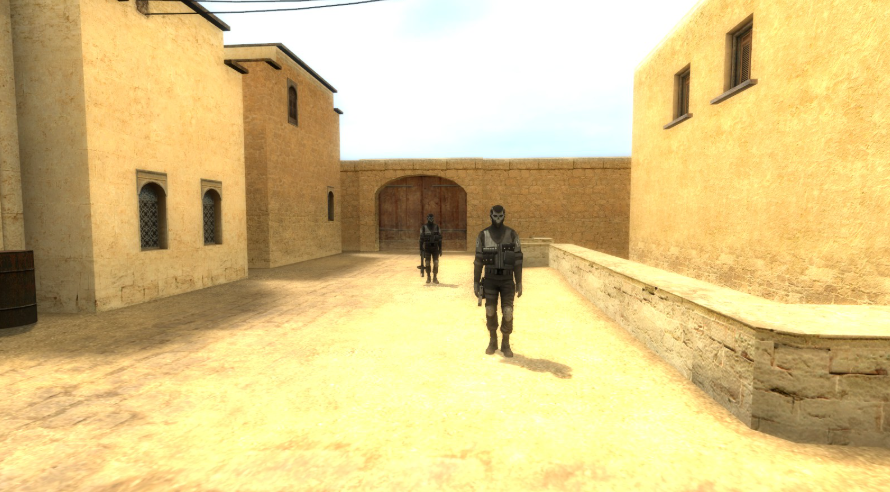
\includegraphics[width=0.6\textwidth]{../fotos/vijand.png}
    \caption{Voorbeeld van datasetfoto}
    \label{fig:vijand}
\end{figure}

Deze beelden werden vervolgens geüpload naar Roboflow. Het is mogelijk om in roboflow handmatig de bounding boxes te tekenen over elke foto maar roboflow voorziet een model dat automatisch kan detecteren door een prompt te geven naar wat het model moet zoeken. Hierdoor kan er kostbare tijd en energie vermeden worden. Het enigste wat er dan nog moet gebeuren is de controle of het aantal gedetecteerde "soldaten" effectief te zien zijn op de foto.

\begin{figure}[H]
    \centering
    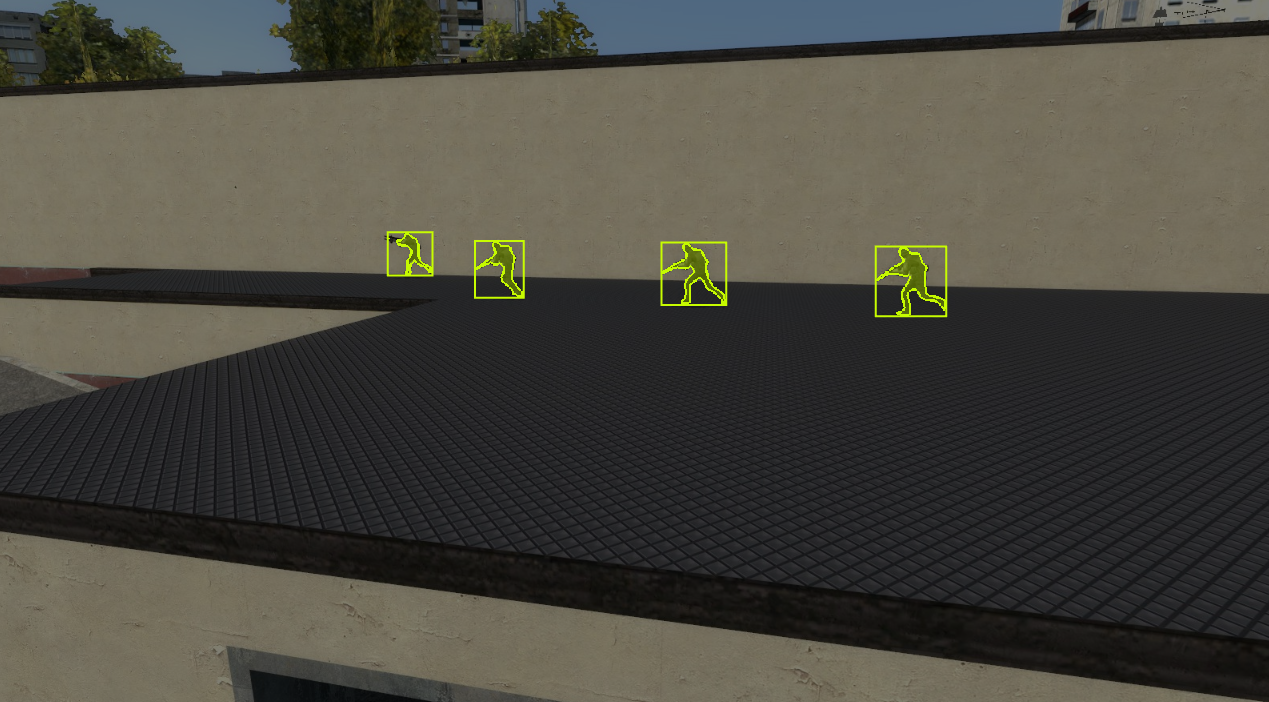
\includegraphics[width=0.8\textwidth]{../fotos/annotatie.png}
    \caption{Voorbeeld van annotatie}
    \label{fig:annotatie}
\end{figure}

Deze annotaties vormen de \textit{ground truth} waarop het model getraind wordt.
\newpage
\section{Dataset preprocessing en augmentatie}

Om de robuustheid van het model te verhogen, werd gebruikgemaakt van data augmentatie. Hierbij worden automatisch variaties van bestaande afbeeldingen gegenereerd.

Enkele voorbeelden van toegepaste augmentaties zijn:
\begin{itemize}
    \item horizontale spiegeling;
    \item rotaties;
    \item aanpassing van helderheid en contrast;
    \item lichte vervormingen (scaling en cropping).
\end{itemize}

Het doel van deze technieken is om het model beter te laten generaliseren naar nieuwe, ongeziene situaties.

\begin{figure}[H]
    \centering
    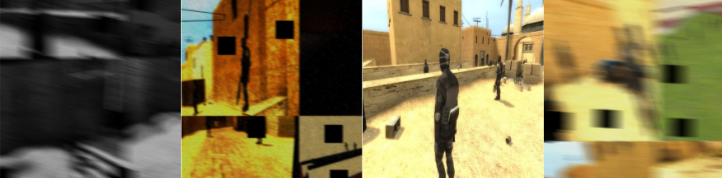
\includegraphics[width=0.8\textwidth]{../fotos/preprocessing.png}
    \caption{Voorbeeld van preprocessing}
    \label{fig:preprocessing}
\end{figure}

Daarnaast kan je de dataset opsplitsen in training, validatie en test sets.
\begin{itemize}
    \item \textbf{Training set (70\%)}: voor het trainen van het model;
    \item \textbf{Validation set (20\%)}: voor het afstellen van hyperparameters;
    \item \textbf{Test set (10\%)}: voor evaluatie van prestaties.
\end{itemize}
\newpage
\section{Modeltraining}

Voor de effectieve training werd gebruikgemaakt van een YOLO-gebaseerd model (\textit{You Only Look Once}), dat geschikt is voor real-time objectdetectie.

Tijdens de training leert het model een functie:

\[
f(I) \rightarrow \{B_1, B_2, ..., B_n\}
\]

waarbij:
\begin{itemize}
    \item \(I\) een inputbeeld is;
    \item \(B_i\) de gedetecteerde bounding boxes voorstellen.
\end{itemize}

Het model optimaliseert zijn parameters door het minimaliseren van een verliesfunctie (\textit{loss function}), die typisch bestaat uit:
\begin{itemize}
    \item classificatiefout (is dit een vijand of niet?);
    \item lokalisatiefout (hoe goed ligt de bounding box?);
    \item confidence score (hoe zeker is het model?).
\end{itemize}

\section{Export en integratie}

Na het trainen werd het model geëxporteerd vanuit Roboflow naar een formaat dat geschikt is voor verdere verwerking (bijvoorbeeld PyTorch of ONNX).

Dit model kan vervolgens gebruikt worden in een realtime pipeline waarbij:
\begin{enumerate}
    \item videoframes worden ingelezen;
    \item het model vijanden detecteert;
    \item de output wordt omgezet naar schermcoördinaten.
\end{enumerate}

Deze output vormt de basis voor verdere verwerking, zoals het berekenen van muisbewegingen binnen het systeem.

\section{Conclusie}

Door gebruik te maken van Roboflow kon het volledige proces van datasetcreatie, annotatie en training efficiënt uitgevoerd worden.

Het resulterende model is in staat om vijanden in realtime te detecteren en vormt een cruciale component binnen de verdere ontwikkeling van het systeem.